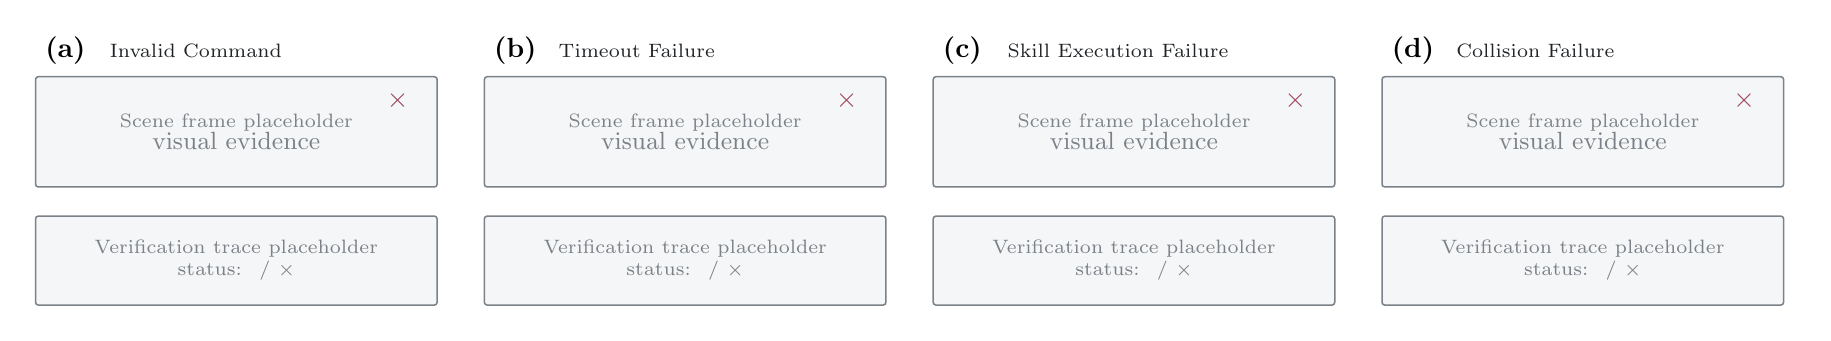
\begin{tikzpicture}[x=1cm,y=1cm,font=\rmfamily\fontsize{7.3}{8.1}\selectfont]
  \definecolor{ink}{HTML}{202326}
  \definecolor{border}{HTML}{7A8188}
  \definecolor{fail}{HTML}{9A435A}
  \definecolor{fill}{HTML}{F5F6F7}
  \foreach \x/\tag/\name in {0/{(a)}/{Invalid Command},5.7/{(b)}/{Timeout Failure},11.4/{(c)}/{Skill Execution Failure},17.1/{(d)}/{Collision Failure}}{
    \begin{scope}[shift={(\x,0)}]
      \node[anchor=west,font=\bfseries] at (0.10,3.28) {\tag};
      \node[anchor=west,text=ink] at (0.92,3.28) {\name};
      \draw[border,fill=fill,rounded corners=1pt,line width=0.55pt]
        (0.10,1.55) rectangle (5.20,2.95);
      \node[text=border,align=center] at (2.65,2.25) {Scene frame placeholder\\\small visual evidence};
      \draw[border,fill=fill,rounded corners=1pt,line width=0.55pt]
        (0.10,0.05) rectangle (5.20,1.18);
      \node[text=border,align=center] at (2.65,0.62) {Verification trace placeholder\\status: $\checkmark$ / $\times$};
      \node[text=fail,font=\bfseries] at (4.70,2.65) {$\times$};
    \end{scope}
  }
  \path[use as bounding box] (0.0,-0.05) rectangle (22.55,3.55);
\end{tikzpicture}
